\chapter{Implementing the Metropolis Acceptance Criteria}

All Monte Carlo moves are implemented in Cassandra to preserve detailed balance between each pair of microstates $m$ and $n$
\begin{equation}
\label{eq:detailedBalance}
\Pi_{mn}\ \alpha_{mn}\ p_m = \Pi_{nm}\ \alpha_{nm}\ p_n
\end{equation}
where $\Pi_{mn}$ is the probability of accepting the move from microstate $m$ to microstate $n$, $\alpha_{mn}$ is the probability of attempting the move that will form $n$ from $m$, and $p_m$ is the probability of $m$ in the ensemble of interest.

In Cassandra, detailed balance is enforced via the Metropolis criterion
\begin{equation}
\label{eq:metropolis}
\Pi_{mn} = \min\left(1, \frac{\alpha_{nm}}{\alpha_{mn}} \frac{p_n}{p_m} \right)
\end{equation}
The ratio in Eq.\ (\ref{eq:metropolis}) will often involve an exponential, e.g. $e^{-\beta \Delta U}$. To preserve precision in the energy calculation, the acceptance probability is computed
\begin{equation}
\label{eq:metropolis_2}
\Pi_{mn} = \exp\left\{-\max\left[0, \ln\left(\frac{\alpha_{mn}}{\alpha_{nm}} \frac{p_m}{p_n}\right)\right]\right\}
\end{equation}
The logarithm, defined in code as ln\_pacc, is tested in the function accept\_or\_reject() which is defined in file accept\_or\_reject.f90. If ln\_pacc is greater than 0 and less than a maximum numerical value, $\Pi_{mn}$ is computed and compared to a random number.

\begin{minipage}{\linewidth}
\begin{lstlisting}[firstnumber=47, caption=accept\_or\_reject.f90]
  accept = .FALSE.

  IF (ln_pacc <= 0.0_DP) THEN

     accept = .TRUE.

  ELSE IF ( ln_pacc < max_kBT) THEN

     pacc = DEXP(-ln_pacc)

     IF ( rranf() <= pacc ) THEN
         
        accept = .TRUE.

     END IF

  END IF
\end{lstlisting}
\end{minipage}

\section{Canonical Monte Carlo}
\label{sec:NVT}
In the canonical ensemble, the number of molecules $N$, the volume $V$ and temperature $T$ are all constant. The position, orientation and conformation of a semi-flexible molecule with fixed bond-lengths containing $M$ atoms is given by a 2$M$+1-dimensional vector $\mathbf{q}$. The positions, orientations and conformations of all $N$ molecules are denoted $\mathbf{q}^N$.

The probability of observing microstate $m$ with configuration $\mathbf{q}_m^N$ is
\begin{equation}
\label{eq:pNVT}
p_m = \frac{e^{-\beta U\left(\mathbf{q}_m^N\right)}}{Z(N,V,T)}\ d\mathbf{q}^N
\end{equation}
where $\beta$ is the inverse temperature $1/k_BT$, $U$ is the potential energy, the differential volume $d\mathbf{q}^N$ is included to make $p_m$ dimensionless and $Z$ is the configurational partition function
\begin{equation}
\label{eq:configPartitionFn_NVT}
Z(N,V,T) = \int e^{-\beta U(\mathbf{q}^N)} d\mathbf{q}^N.
\end{equation}
The integral is over all $N(2M+1)$ degrees of freedom. The ratio of microstate probabilities follows from Eq.\ (\ref{eq:pNVT})
\begin{align}
\label{eq:pNVT_ratio}
\frac{p_m}{p_n} &= \frac{e^{-\beta U\left(\mathbf{q}_m^N\right)} d\mathbf{q}^N/Z(N,V,T)}{e^{-\beta U\left(\mathbf{q}_n^N\right)} d\mathbf{q}^N/Z(N,V,T)} \nonumber \\
&= e^{\beta (U_n - U_m)} = e^{\beta \Delta U}
\end{align}
The configurational partition function $Z$ and differential volume $d\mathbf{q}^N$ both cancel, leaving only the ratio of Boltzmann factors.

New configurations are generated by attempting moves that translate, rotate and regrow a randomly selected molecule.

\subsection{Translating a Molecule}
\label{sec:translate}
A molecule is translated by moving its center of mass in each Cartesian direction by a random amount chosen from the uniform distribution on the interval [-$\delta r_{max},\delta r_{max}$]. The maximum displacement $\delta r_{max}$ must be given in the input file. The translation move is symmetric in forward and reverse directions. That is, either microstate $n$ can be formed from microstate $m$ and vice versa by moving one molecule within $\delta r_{max}$ in each Cartesian direction, or microstate $n$ cannot be formed at all. As a result, $\alpha_{mn} = \alpha_{nm}$.

The acceptance probability for a translation move follows from Eq.\ (\ref{eq:pNVT_ratio})
\begin{equation}
\label{eq:pAcc_translate}
\ln \left( \frac{\alpha_{mn}}{\alpha_{nm}} \frac{p_m}{p_n} \right) = \ln \left( \frac{p_m}{p_n} \right) = \beta \Delta U
\end{equation}

In Cassandra, the translation move is implemented in the subroutine Translate defined in translate.f90. The relevant lines from version 1.1 are quoted below. The variable names in the translate.f90 code are identified with the symbols from Eq.\ (\ref{eq:pAcc_translate}) in Table \ref{table:translate}.

\begin{lstlisting}[firstnumber=274, caption=translate.f90, label=code:translate]
ln_pacc = beta(this_box) * delta_e
accept = accept_or_reject(ln_pacc)
\end{lstlisting}

\begin{table}
\caption{Variable symbols and code names for translating and rotating a molecule}
\label{table:translate}
\centering
\begin{tabular}{|c|c|} \hline
 {\bf Symbol} & {\bf Code name} \\ \hline
 $\beta$ & beta(this\_box) \\
 $\Delta U$ & delta\_e \\
 \hline
\multicolumn{2}{c}{}
\end{tabular}
\end{table}

\subsection{Rotating a Molecule}
\label{sec:rotate}
A linear molecule is rotated differently than a nonlinear molecule. A molecule is identified as linear if it is composed of 2 atoms or if all the angles are rigid with a bond angle of 180$\degree$. If the molecule is linear: 

\begin{enumerate}
	\item Pick three random angles: $\phi$ on [$-\pi,\pi$], $\cos(\theta)$ on [-1,1], and $\psi$ on [$-\pi,\pi$].
	\item With the origin at the molecule's center of mass, rotate by $\phi$ around $z$, rotate by $\theta$ around $x'$, and rotate by $\psi$ around $z'$, as shown in Fig. \ref{fig:EulerAngles}.
\end{enumerate}

Even though three angles are randomly chosen, the probability of the resulting orientation is $d\cos(\theta)d\phi/4\pi$.

\begin{figure}[h]
	\centering
	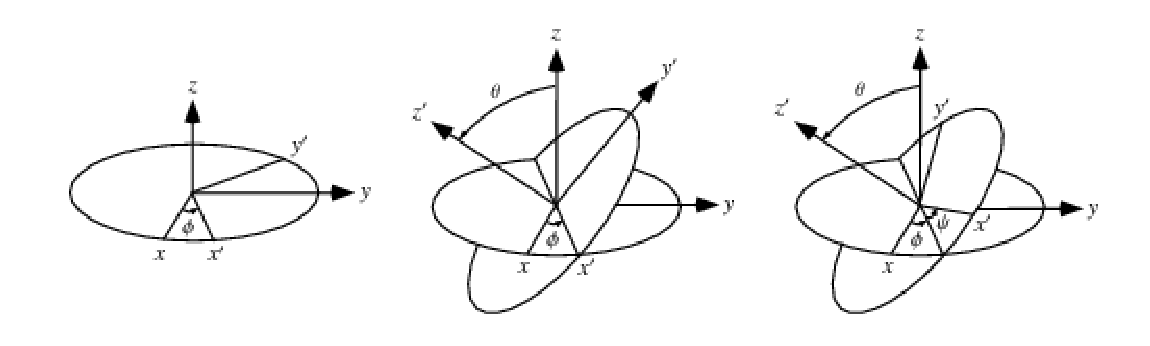
\includegraphics[width=0.9\textwidth]{EulerAngles.eps}
	\caption{Procedure for rotating linear molecules. \newline Image from mathworld.wolfram.com/EulerAngles.html.}
	\label{fig:EulerAngles}
\end{figure}

If the molecule is nonlinear:

\begin{enumerate}
	\item Randomly select an axis: $x$, $y$, or $z$.
	\item Choose a random angular displacement $\delta \theta$ from $[-\delta \theta_{max}, \delta \theta_{max}]$. $\delta \theta_{max}$ must be given in the input file.
	\item Rotate the molecule around a vector parallel to the selected axis and through its center of mass by $\delta \theta$.
\end{enumerate}

In either case, the rotation move is symmetric, $\alpha_{mn} = \alpha_{nm}$, and the acceptance criteria is given by Eq.\ (\ref{eq:pAcc_translate}). The rotation move is implemented in subroutine Rotate defined in rotate.f90.

\begin{lstlisting}[firstnumber=261, caption=rotate.f90, label=code:rotate]
ln_pacc = beta(this_box) * delta_e
accept = accept_or_reject(ln_pacc)
\end{lstlisting}

\subsection{Regrowing a Molecule}
\label{sec:regrow}
Internal degrees of freedom in flexible molecules are sampled by deleting one or more fragments from the molecule and replacing the deleted fragments with conformations from a reservoir of fragment conformations. If the molecule consists of only a single fragment (e.g, water, all atom methane, united atom propane, all atom cyclohexane), the entire molecule is deleted and replaced as follows:

\begin{enumerate}
	\item Randomly select a molecule $i$ with uniform probability $1/N$, record its center-of-mass position and delete it.
	\item Select a molecular conformation with Boltzmann probability $e^{-\beta U(\mathbf{q}_{int,n}^{(i)})}/Z_{int}$, where $\mathbf{q}_{int,n}^{(i)}$ are the internal bond or improper angles of molecule $i$ in microstate $n$ and $Z_{int}$ is the configurational partition function over internal degrees of freedom (see Eq. (\ref{eq:configPartitionFn_1VT})).
	\item Pick three random angles: $\phi$ on [$-\pi,\pi$], $\cos(\theta)$ on [-1,1], and $\psi$ on [$-\pi,\pi$]. Rotate the molecule as shown in Fig. \ref{fig:EulerAngles}. The probability of the resulting orientation is $d\mathbf{q}_{rot}/Z_{rot}$, which for a nonlinear molecule is $d\cos(\theta) d\phi d\psi / 8 \pi^2$.
	\item Place the molecule with the selected conformation and orientation at the same center-of-mass position as the deleted molecule.
\end{enumerate}

Regrowing a monoatomic particle has no effect. Regrowing a linear molecule is the same as rotating it. The overall probability $\alpha_{mn}$ of regrowing a molecule with the selected orientation and conformation is 

\begin{equation}
\label{eq:alpha_regrow}
\alpha_{mn} = \frac{1}{N} \frac{d\mathbf{q}_{rot}}{Z_{rot}} \frac{e^{-\beta U(\mathbf{q}_n^{(i)})}d\mathbf{q}_{int}}{Z_{int}}
\end{equation}

where $\mathbf{q}_n^{(i)}$ denotes the position, orientation and conformation of molecule $i$ in microstate $n$ and $U(\mathbf{q}_n^{(i)})$ is the potential energy of the isolated molecule $i$, i.e. the intramolecular potential energy. The reverse probability $\alpha_{nm}$ is identical except for the intramolecular potential energy $U(\mathbf{q}_m^{(i)})$ of molecule $i$ in microstate $m$. Using Eqs. (\ref{eq:pNVT_ratio}) and (\ref{eq:alpha_regrow}), the acceptance criteria for the regrowth of a single fragment molecule is

\begin{align}
\label{eq:pAcc_regrow}
\ln\left( \frac{\alpha_{mn}}{\alpha_{nm}} \frac{p_m}{p_n} \right) &= \beta \left[\left(U(\mathbf{q}^N_n) - U(\mathbf{q}^N_m)\right) - \left( U(\mathbf{q}_n^{(i)}) - U(\mathbf{q}_m^{(i)})\right)\right] \\ \nonumber
&= \beta \Delta U - \beta \Delta U_{int}^{(i)} = \beta \Delta U_{inter}^{(i)}
\end{align}

Only the change in the intermolecular potential energy between molecule $i$ and the other $N-1$ molecules contributes to the acceptance criteria. The code that implements Eq. (\ref{eq:pAcc_regrow}) is shown in Code \ref{code:cbmcRegrow} in Section \ref{sec:cbmcRegrow}.

If the molecule consists of more than one fragment (e.g., all atom ethane, all atom toluene, united atom butane), a bond is cut and the severed fragments are regrown using Configurational Bias Monte Carlo (CBMC). See Section \ref{sec:cbmcRegrow} for more details.

\subsection{Canonical Partition Function}
In Sections \ref{sec:translate}-\ref{sec:rotate}, the microstate probability is normalized by the configuration partition function $Z$ because the only relevant degrees of freedom are configurational. In other ensembles, the full partition function $Q$ appears, integrated over both configuration space $\mathbf{q}^N$ and momenta space $\mathbf{p}_q^N$

\begin{equation}
\label{eq:partitionFn_NVT}
Q(N,V,T) = \frac{1}{h^{N(2M+1)} N!} \int e^{-\beta H(\mathbf{p}_q^N, \mathbf{q}^N)}\ d\mathbf{p}_q^N d\mathbf{q}^N
\end{equation}

where the 2$M$+1 momenta $\mathbf{p}_q$ are conjugate to the generalized coordinates $\mathbf{q}$. The momenta and configuration integrals are separable, and the single molecule momenta integrals are all identical.

\begin{align}
Q(N,V,T) &= \frac{1}{N!} \left[\int e^{-\beta U(\mathbf{q}^N)} d\mathbf{q}^N \right] \left[\frac{1}{h^{2M+1}} \int e^{-\beta K(\mathbf{p}_q)}\ d\mathbf{p}_q \right]^N \nonumber \\
&= \frac{1}{N!} Z(N,V,T) \left[\frac{Q(1,V,T)}{Z(1,V,T)}\right]^N
\end{align}

where $Q(1,V,T)$ is the partition function of a single molecule in a box. The center of mass integrals for a single molecule are separable from the integrals over rotational and internal degrees of freedom:

\begin{equation}
\label{eq:partitionFn_1VT}
Q(1,V,T) = Q_{com}Q_{rot+int} = V \Lambda^{-3} Q_{rot+int}
\end{equation}

where $\Lambda$ is the de Broglie wavelength of the molecule and the rotational and internal momenta integratals in $Q_{rot+int}$ are not separable since the moments of inertia will depend on the conformation adopted by the molecule. The configurational partition function is further separable into center of mass (translational), orientational and internal degrees of freedom:

\begin{equation}
\label{eq:configPartitionFn_1VT}
Z(1,V,T) = VZ_{rot}Z_{int}
\end{equation}

where the volume $V$ is the translational partition function and $Z_{rot}$ equals 4$\pi$ for a linear molecule and 8$\pi^2$ for a nonlinear molecule.

\section{Isothermal-Isobaric Monte Carlo}
\label{sec:NPT}
In the isothermal-isobaric ensemble, the number of particles $N$, the pressure $P$ and temperature $T$ are all constant while the volume $V$ and energy $E$ fluctuate. The partition function is

\begin{equation}
\label{eq:partitionFn_NPT}
\Delta(N,P,T) = \int e^{-\beta P V} Q(N,V,T) dV
\end{equation}

Note that $Q$ is dimensionless and $\Delta$ has dimensions of volume. The probability of the system having volume $V$ is 

\begin{equation}
\label{eq:pV}
p(V) = \frac{Q(N,V,T)e^{-\beta P V}}{\Delta(N,P,T)}dV
\end{equation}

The probability of observing microstate $m$ with configuration $\mathbf{q}_m^N$ and volume $V_m$ is

\begin{align}
\label{eq:pNPT}
p_m &= \frac{e^{-\beta U(\mathbf{q}_m^N)}d\mathbf{q}_m^N}{Z(N,V_m,T)}\ \frac{Q(N,V_m,T) e^{-\beta P V_m} dV}{\Delta(N,P,T)} \nonumber \\
&= \frac{e^{-\beta U_m - \beta P V_m}}{\Delta(N,P,T)}\ \left(\frac{Q(1,V_m,T)}{Z(1,V_m,T)}\ d\mathbf{q}_m\right)^N dV
\end{align}

where the differential volume element $d\mathbf{q}_m^N$ has subscript $m$ becuase it depends on the volume $V_m$. The ratio of microstate probabilities is

\begin{equation}
\label{eq:pNPT_ratio}
\frac{p_m}{p_n} = e^{\beta (U_n - U_m) + \beta P (V_n - V_m)} \left(\frac{d\mathbf{q}_m}{d\mathbf{q}_n}\right)^N = e^{\beta \Delta U + \beta P \Delta V} \left(\frac{d\mathbf{q}_m}{d\mathbf{q}_n}\right)^N
\end{equation}

\subsection{Scaling the Volume}
\label{subsec:scaling_the_volume}
In Cassandra, new volumes are sampled as follows:

\begin{enumerate}
	\item Pick a random volume $\Delta V$ with uniform probability from the interval [$-\delta V_{max}$,\ $\delta V_{max}$]. The trial volume is $V + \Delta V$.
	\item Scale the box lengths uniformly.
	\item Scale the center of mass of each molecule uniformly.
\end{enumerate}

The probability of selecting $\Delta V$ is the same as selecting $-\Delta V$ which makes scaling the volume symmetric, $\alpha_{mn}=\alpha_{nm}$. Scaling the configurations changes the differential element $d\mathbf{q}_m^N$ surrounding configuration $\mathbf{q}_m^N$. Only the molecular centers of mass change, so we can separate $d\mathbf{q}$ into 3 center of mass coordinates $d\mathbf{r}_{com}$ and 2$M$-2 orientational and internal coordinates $d\mathbf{q}_{rot+int}$. The scaled center of mass positions are held constant, making $d\mathbf{r}_{com} = V d\mathbf{s}_{com}$. The acceptance probability for a volume scaling move is

\begin{equation}
\label{eq:pAcc_volume}
\ln \left( \frac{\alpha_{mn}}{\alpha_{nm}} \frac{p_m}{p_n} \right) = \ln \left( \frac{p_m}{p_n} \right) = \beta \Delta U + \beta P \Delta V + N \ln\left(\frac{V_m}{V_n}\right)
\end{equation}

The volume scaling move is implemented in subroutine Volume\_Change defined in volume\_change.f90. 

\begin{lstlisting}[firstnumber=475, caption=volume\_change.f90, label=code:volume]
ln_pacc = beta(this_box) * delta_e &
        + beta(this_box) * pressure(this_box) * delta_volume &
        - total_molecules * DLOG(box_list(this_box)%volume/box_list_old%volume)
accept = accept_or_reject(ln_pacc)
\end{lstlisting}

\begin{table}
\caption{Variable symbols and code names for volume scaling move.}
\label{table:volume}
\centering
\begin{tabular}{|c|c|} \hline
 {\bf Symbol} & {\bf Code name} \\ \hline
 $\beta$ & beta(this\_box) \\
 $\Delta U$ & delta\_e \\
 $P$ & pressure(this\_box) \\
 $\Delta V$ & delta\_volume \\
 $N$ & total\_molecules \\
 $V_n$ & box\_list(this\_box)\%volume \\
 $V_m$ & box\_list\_old\%volume \\
 \hline
\multicolumn{2}{c}{}
\end{tabular}
\end{table}


\section{Grand Canonical Monte Carlo}
\label{sec:MuVT}
In the grand canonical ensemble, the chemical potential $\mu$, the volume $V$ and temperature $T$ are held constant while the number of molecules $N$ and energy $E$ fluctuate. The partition function is 

\begin{equation}
\label{eq:partitionFn_MuVT}
\Xi(\mu,V,T) = \sum\limits_{N=0}^{\infty} Q(N,V,T)\ e^{\beta \mu N}
\end{equation}

The probability of the system having $N$ molecules is 

\begin{equation}
\label{eq:pN}
p(N) = \frac{Q(N,V,T)e^{\beta \mu N}}{\Xi(\mu,V,T)}
\end{equation}

The probability of observing microstate $m$ with $N_m$ molecules and configuration $\mathbf{q}_m^{N_m}$ is

\begin{align}
\label{eq:pMuVT}
p_m &= \frac{e^{-\beta U(\mathbf{q}_m^{N_m})} d\mathbf{q}^{N_m}}{Z(N_m,V,T)}\ \frac{Q(N_m,V,T)e^{\beta \mu N_m}}{\Xi(\mu,V,T)} \nonumber \\
&= \frac{e^{-\beta U_m + \beta \mu N_m}}{\Xi(\mu,V,T)}\ \left[\frac{Q(1,V,T)}{Z(1,V,T)}\ d\mathbf{q}\right]^{N_m}
\end{align}

Note that Eq.\ (\ref{eq:pMuVT}) does not contain the factorial $N_m!$ that accounts for indistinguishable particles. In a simulation, particles {\em are} distinguishable: they are numbered and specific particles are picked for MC moves. The ratio of microstate probabilities is

\begin{equation}
\label{eq:pMuVT_ratio}
\frac{p_m}{p_n} = e^{\beta \Delta U - \beta \mu \Delta N}\ \left[\frac{Q(1,V,T)}{Z(1,V,T)}\ d\mathbf{q}\right]^{-\Delta N}
\end{equation}

Alternatively, Eq.\ (\ref{eq:pMuVT_ratio}) can be recast to use the fugacity $f$ instead of the chemical potential $\mu$. The relationship between $\mu$ and $f$ is

\begin{equation}
\label{eq:mu}
\mu = -k_BT \ln\left( \frac{Q(1,V,T)}{N} \right) = -k_BT\ \ln\left( \frac{Q(1,V,T)}{\beta f V} \right)
\end{equation}

Inserting Eq.\ (\ref{eq:mu}) into Eq.\ (\ref{eq:pMuVT_ratio}) yields

\begin{equation}
\label{eq:pfVT_ratio}
\frac{p_m}{p_n} = e^{\beta \Delta U}\ \left[\frac{\beta f V}{Z(1,V,T)}\ d\mathbf{q}\right]^{-\Delta N}
\end{equation}


Fluctuations in the number of molecules are achieved by inserting and deleting molecules. A successful insertion increases the number of molecules from $N$ to $N$ + 1, i.e. $\Delta N = 1$. A successful deletion decreases the number of molecules from $N$ to $N$ - 1, i.e. $\Delta N = -1$. 

Random insertions and deletions (see Section \ref{sec:appendix}) in the liquid phase typically have very high $\Delta U$ due to core overlap and dangling bonds, respectively, making the probability of acceptance very low. Instead, insertions in Cassandra are attempted using Configurational Bias Monte Carlo.

\subsection{Inserting a Molecule with \newline Configurational Bias Monte Carlo}
\label{sec:cbmcInsert}

In Configurational Bias Monte Carlo (CBMC), the molecular conformation of the inserted molecule is molded to the insertion cavity. First, the molecule is parsed into fragments such that each fragment is composed of (a) a central atom and the atoms directly bonded to it (see Fig. \ref{fig:propaneFragments}), or (b) a ring of atoms and all the atoms directly bonded to them. Then, a position, orientation and molecular conformation of the molecule to be inserted are selected via the following steps:

\begin{figure}[h]
	\centering
	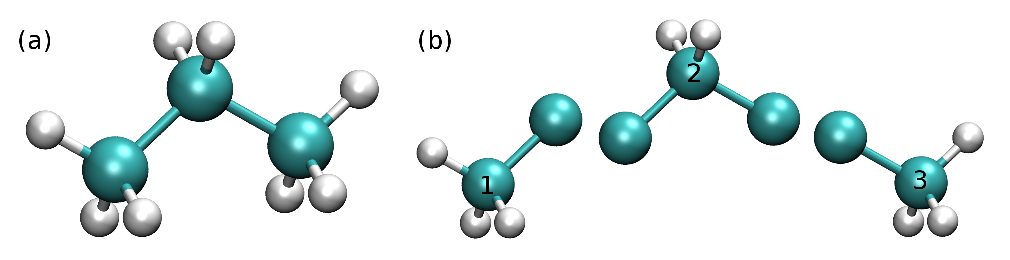
\includegraphics[width=0.99\textwidth]{c3.eps}
	\caption{(a) An all-atom model of propane. (b) The same model as in (a), but parsed into three fragments.}
	\label{fig:propaneFragments}
\end{figure}


\begin{enumerate}
  \item Select the order in which each fragment of the ($N+1$)th molecule will be placed. The probability of the resulting sequence is $p_{seq}$. (See example in Table. \ref{table:propane}.)
  \begin{enumerate}
		\item The first fragment $i$ is chosen with uniform probability 1/$N_{frag}$.
    \item Subsequent fragments must be connected to a previously chosen fragment and are chosen with the uniform probability 1/$N_{cnxn}$, where the number of connections $N_{cnxn}= \sum_{ij}{\delta_{ij} h_{i} (1-h_{j})}$ is summed over all fragments $i$ and $j$. $h_i$ is 1 if fragment $i$ has been previously chosen and 0 otherwise. $\delta_{ij}$ is 1 if fragments $i$ and $j$ are connected and 0 otherwise.
  \end{enumerate}
	\item Select a conformation for fragment $i$ with Boltzmann probability \newline $e^{-\beta U(\mathbf{q}_{frag_i})}d\mathbf{q}_{frag_i}/Z_{frag_i}$, where $\mathbf{q}_{frag_i}$ are the internal degrees of freedom (angles and/or impropers) associated with fragment $i$.
	\item Select an orientation with uniform probability $d\mathbf{q}_{rot}/Z_{rot}$. 
	\item Select a coordinate for the center of mass (COM) of fragment $i$:
	\begin{enumerate}
		\item Select $\kappa_{ins}$ trial coordinates $\mathbf{r}_k$, each with uniform probability $d\mathbf{r}/V$. Since one of the trial coordinates will be selected later, the individual probabilities are additive. The probability of the collection of trial coordinates is $\kappa_{ins}d\mathbf{r}/V$.
		\item Compute the change in potential energy $\Delta U_k^{ins}$ of inserting fragment $i$ at each position $\mathbf{r}_k$ into configuration $\mathbf{q}_m^N$.
		\item Select one of the trial coordinates with probability $e^{-\beta \Delta U_k^{ins}} / \sum_k{e^{-\beta \Delta U_k^{ins}}}$.
	\end{enumerate}
	\item For each additional fragment $j$:
	\begin{enumerate}
		\item Select a fragment conformation with Boltzmann probability\newline$e^{-\beta U(\mathbf{q}_{frag_j})}d\mathbf{q}_{frag_j}/Z_{frag_j}$
		\item Select the first of $\kappa_{dih}$ trial dihedrals $\phi_0$ with uniform probability from the interval [0,$\frac{2\pi}{\kappa_{dih}}$). Additional trial dihedrals are equally spaced around the unit circle, $\phi_k=\phi_{k-1}+2\pi/\kappa_{dih}$. The probability of selecting $\phi_0$ is $\kappa_{dih}d\phi/2\pi$.
		\item Compute the change in potential energy $\Delta U_k^{dih}$ of attaching fragment $j$ to the growing molecule with each dihedral $\phi_k$.
		\item Select one of the trial dihedrals with probability $e^{-\beta \Delta U_k^{dih}} / \sum_k{e^{-\beta \Delta U_k^{dih}}}$.
	\end{enumerate}
\end{enumerate}

\begin{table}
\caption{Possible sequences and probabilities for inserting the fragments of the all-atom model of propane shown in Fig. \ref{fig:propaneFragments}.}
\label{table:propane}
\centering
\begin{tabular}{|c|c|} \hline
 {\bf Sequence} & {\bf $p_{seq}$} \\ \hline
 1 2 3 & 1/3 \\
 2 1 3 & 1/6 \\
 2 3 1 & 1/6 \\
 3 2 1 & 1/3 \\
 \hline
\multicolumn{2}{c}{}
\end{tabular}
\end{table}

The overall probability $\alpha_{mn}$ of attempting the insertion with the selected position, orientation and conformation is 

\begin{align}
\alpha_{mn} &= p_{seq}\ \frac{d\mathbf{q}_{rot}}{Z_{rot}}\ \frac{\kappa_{ins}d\mathbf{r}}{V}\ \frac{e^{-\beta \Delta U_k^{ins}}}{\sum_k{e^{-\beta \Delta U_k^{ins}}}}\ \times \nonumber \\
&\ \ \ \left[\prod_{i=1}^{N_{frag}}{\frac{e^{-\beta U(\mathbf{q}_{frag_i})}d\mathbf{q}_{frag_i}}{Z_{frag_i}}}\right]\ \left[\prod_{j=1}^{N_{frag}-1}{\frac{\kappa_{dih}d\phi}{2\pi}\ \frac{e^{-\beta \Delta U_k^{dih}}}{\sum_k{e^{-\beta \Delta U_k^{dih}}}}}\right] \\
\label{eq:alpha_cbmcInsert}
&= p_{seq}\ p_{bias}\ \frac{e^{-\beta U(\mathbf{q}_{frag})}d\mathbf{q}}{VZ_{rot}Z_{frag}\Omega_{dih}}
\end{align}

where $Z_{frag} = \prod_i Z_{frag_i}$ is the configurational partition function over degrees of freedom internal to each fragment, $U(\mathbf{q}_{frag}) = \sum_iU(\mathbf{q}_{frag_i})$ is the summed potential energy of each of the (disconnected) fragments, $\Omega_{dih} = (2\pi)^{N_{frag}-1}$ and $p_{bias}$ is

\begin{equation}
p_{bias} = \frac{\kappa_{ins}\ e^{-\beta \Delta U_k^{ins}}}{\sum_k{e^{-\beta \Delta U_k^{ins}}}}\ \left[\prod_{j=1}^{N_{frag}-1}{\frac{\kappa_{dih}\ e^{-\beta \Delta U_k^{dih}}}{\sum_k{e^{-\beta \Delta U_k^{dih}}}}}\right]
\end{equation}

Note that the term $VZ_{rot}Z_{frag}\Omega_{dih}$ in the denominator of Eq.\ (\ref{eq:alpha_cbmcInsert}) differs from $Z(1,V,T)=VZ_{rot}Z_{int}$.

In the reverse move, 1 of the $N+1$ particles is randomly selected for deletion. The probability $\alpha_{nm}$ of picking the molecule we just inserted is

\begin{equation}
\label{eq:alpha_cbmcReverseInsert}
\alpha_{nm} = \frac{1}{N+1}
\end{equation}

Combining Eqs.\ (\ref{eq:alpha_cbmcInsert}) and (\ref{eq:alpha_cbmcReverseInsert}) with Eq.\ (\ref{eq:pMuVT_ratio}) or Eq.\ (\ref{eq:pfVT_ratio}) gives the acceptance probability for a CBMC insertion move

\begin{align}
\label{eq:pAcc_cbmcInsertMuShift}
\ln\left( \frac{\alpha_{mn}}{\alpha_{nm}} \frac{p_m}{p_n} \right) &= \beta \left[\Delta U - U(\mathbf{q}^{(N+1)}_{frag,n})\right] - \beta \mu' + \ln\left( \frac{(N+1)\Lambda^3}{V} \right) + \ln\left( p_{seq}p_{bias} \right) \\
\label{eq:pAcc_cbmcInsertFShift}
&= \beta \left[\Delta U - U(\mathbf{q}^{(N+1)}_{frag,n})\right] + \ln\left( \frac{N+1}{\beta f' V} \right) + \ln\left( p_{seq}p_{bias} \right)
\end{align}

where $\mu'$ and $f'$ are, respectively, a shifted chemical potential and a skewed fugacity,

\begin{align}
\label{eq:muShift}
\mu'&=\mu+k_BT\ln\left( Q_{rot+int} \frac{Z_{frag}\Omega_{dih}}{Z_{int}} \right) \\
\label{eq:fShift}
f'&= f \frac{Z_{frag}\Omega_{dih}}{Z_{int}}
\end{align}

All of the terms in Eqs.\ (\ref{eq:muShift}) and (\ref{eq:fShift}) are intensive. GCMC simulations using Eqs.\ (\ref{eq:pAcc_cbmcInsertMuShift}) and (\ref{eq:pAcc_cbmcInsertFShift}) will converge to the same average density regardless of the simulation volume $V$. However, the values of $\mu'$ or $f'$ that correspond to the converged density will {\em not} match tabulated values of $\mu$ or $f$ computed from experimental data.

Note that the term $Z^{IG}/\Omega$ from Macedonia {\em et al}. would be equivalent to $Z_{int}/\Omega_{frag}\Omega_{dih}$ in the nomenclature used here. The configurational partition function of the disconnected fragments integrates over a Boltzmann factor, $Z_{frag} = \int e^{-\beta U(\mathbf{q}_{frag})} d\mathbf{q}_{frag}$, whereas the term $\Omega_{frag} = \int d\mathbf{q}_{frag}$ does not.

In Cassandra, the insertion move is implemented in the subroutine Insertion in insertion.f90. The relevant lines from version 1.1 are quoted below. The variable names in the insertion.f90 code are identified with symbols in Table \ref{table:cbmcInsert}.

\begin{minipage}{\linewidth}
\begin{lstlisting}[firstnumber=441, caption=insertion.f90]
  ln_pacc = beta(this_box) * (delta_e - E_angle - nrg_ring_frag_tot)
\end{lstlisting}
\begin{lstlisting}[firstnumber=447]
  ln_pacc = ln_pacc + DLOG(P_seq * P_bias) &
                    + DLOG(REAL(nmols(is,this_box)+1,DP)) &
                    - DLOG(box_list(this_box)%volume)

  IF(lchempot) THEN
     ! chemical potential is input
     ln_pacc = ln_pacc - species_list(is)%chem_potential * beta(this_box) &
               + 3.0_DP*DLOG(species_list(is)%de_broglie(this_box))
  ELSE   
     ! fugacity is input
     ln_pacc = ln_pacc - DLOG(species_list(is)%fugacity) &
                       - DLOG(beta(this_box)) &
  END IF 

  accept = accept_or_reject(ln_pacc)
\end{lstlisting}
\end{minipage}

\begin{table}
\caption{Variable symbols and code names for inserting a molecule}
\label{table:cbmcInsert}
\centering
\begin{tabular}{|c|c|} \hline
 {\bf Symbol} & {\bf Code name} \\ \hline
 $\beta$ & beta(this\_box) \\
 $\Delta U$ & delta\_e \\
 $U(\mathbf{q}_{frag})$ & E\_angle + nrg\_ring\_frag\_tot \\
 $p_{seq}$ & P\_seq \\
 $p_{bias}$ & P\_bias \\
 $\mu'$ & species\_list(is)\%chem\_potential \\
 $N$ & nmols(is,this\_box) \\
 $V$ & box\_list(this\_box)\%volume \\
 $\Lambda$ & species\_list(is)\%de\_broglie(this\_box) \\
 $f'$ & species\_list(is)\%fugacity \\
 \hline
\multicolumn{2}{c}{}
\end{tabular}
\end{table}

\subsection{Deleting a Molecule that was Inserted via \newline Configurational Bias Monte Carlo}
\label{sec:cbmcDelete}

The probability $\alpha_{mn}$ of choosing a molecule to delete is

\begin{equation}
\alpha_{mn} = \frac{1}{N}
\end{equation}

The probability of the reverse move $\alpha_{nm}$ requires knowledge of the sequence and biasing probabilities $p_{seq}$ and $p_{bias}$ that would have been used to place the molecule if it was being inserted. $p_{seq}$ and $p_{bias}$ can be calculated using the following procedure:

\begin{enumerate}
  \item Select the fragment order using the same procedure for inserting a molecule. The probability of the resulting sequence is $p_{seq}$.
	\item The first fragment in the sequence is fragment $j$. Calculate the intramolecular potential energy of fragment $j$'s current conformation, $U(\mathbf{q}_{frag_j})$. The probability of this conformation is Boltzmann  $e^{-\beta U(\mathbf{q}_{frag_j})}d\mathbf{q}_{frag_j}/Z_{frag_j}$.
	\item The probability of the fragment's current orientation is $d\mathbf{q}_{rot}/Z_{rot}$. 
	\item Calculate the weight of the fragment's current center of mass (COM) coordinates:
	\begin{enumerate}
		\item Compute the interaction potential energy $\Delta U^{ins}$ between fragment $j$ and the other $N-1$ molecules.
		\item Select $\kappa_{ins}-1$ trial coordinates $\mathbf{r}_k$, each with uniform probability $d\mathbf{r}/V$.
		\item Calculate the weight of the fragment's current COM amongst the trial coordinates, $e^{-\beta \Delta U^{ins}} / \sum_k{e^{-\beta \Delta U_k^{ins}}}$.
	\end{enumerate}
	\item For each additional fragment $j$:
	\begin{enumerate}
		\item Calculate the intramolecular potential energy of fragment $j$'s current conformation, $U(\mathbf{q}_{frag_j})$. The weight of this conformation in the Boltzmann distribution is $e^{-\beta U(\mathbf{q}_{frag_j})}d\mathbf{q}_{frag_j}/Z_{frag_j}$.
		\item Calculate the interaction potential energy $\Delta U^{dih}$ between fragment $j$, on the one hand, and fragments $i$ through $j-1$ and the other $N-1$ molecules.
		\item Calculate the current dihedral $\phi_0$ of fragment $j$. Compute the interaction potential energy $\Delta U_k^{dih}$ at $\kappa_{dih}-1$ trial dihedrals $\phi_k = \phi_{k-1} + 2\pi/\kappa_{dih}$.
		\item Compute the weight of $\phi_0$ amongst the trial dihedrals, $e^{-\beta \Delta U^{dih}}/ \sum_k{e^{-\beta \Delta U_k^{dih}}}$.
	\end{enumerate}
\end{enumerate}

The overall probability $\alpha_{nm}$ is 

\begin{equation}
\label{eq:alpha_cbmcReverseDelete}
\alpha_{nm} = p_{seq}\ p_{bias}\ \frac{e^{-\beta U(\mathbf{q}_{frag})}d\mathbf{q}}{VZ_{rot}Z_{frag}\Omega_{dih}}.
\end{equation}

The acceptance criteria for deleting a molecule inserted via CBMC is

\begin{align}
\label{eq:pAcc_cbmcDeleteMuShift}
\ln\left( \frac{\alpha_{mn}}{\alpha_{nm}} \frac{p_m}{p_n} \right) &= \beta \left[\Delta U + U(\mathbf{q}^{(i)}_{frag,m})\right] + \beta \mu' + \ln\left( \frac{V}{N\Lambda^3} \right) - \ln\left( p_{seq}p_{bias} \right) \\
\label{eq_pAcc_cbmcDeleteF}
&= \beta \left[\Delta U + U(\mathbf{q}^{(i)}_{frag,m})\right] + \ln\left( \frac{\beta f' V}{N} \right) - \ln\left( p_{seq}p_{bias} \right)
\end{align}

In Cassandra, the deletion move is implemented in the subroutine Deletion in deletion.f90. The relevant lines are quoted below. The variable names in deletion.f90 code are identified with symbols in Table \ref{table:cbmcDelete}.

\begin{minipage}{\linewidth}
\begin{lstlisting}[firstnumber=334, caption=deletion.f90]
  ln_pacc = beta(this_box) * (delta_e + E_angle + nrg_ring_frag_tot)
\end{lstlisting}
\begin{lstlisting}[firstnumber=340]
  ln_pacc = ln_pacc - DLOG(P_seq * P_bias) &
                    - DLOG(REAL(nmols(is,this_box),DP)) &
                    + DLOG(box_list(this_box)%volume)
 
  IF(lchempot) THEN
     ! chemical potential is input
     ln_pacc = ln_pacc + beta(this_box) * species_list(is)%chem_potential &
             - 3.0_DP*DLOG(species_list(is)%de_broglie(this_box))
  ELSE
     ! fugacity is input
     ln_pacc = ln_pacc + DLOG(species_list(is)%fugacity) &
                       + DLOG(beta(this_box)) &
  END IF
 
  accept = accept_or_reject(ln_pacc)

\end{lstlisting}
\end{minipage}

\begin{table}
\caption{Variable symbols and code names for deleting a molecule}
\label{table:cbmcDelete}
\centering
\begin{tabular}{|c|c|} \hline
 {\bf Symbol} & {\bf Code name} \\ \hline
 $\beta$ & beta(this\_box) \\
 $\Delta U$ & delta\_e \\
 $U(\mathbf{q}_{frag})$ & E\_angle + nrg\_ring\_frag\_tot \\
 $p_{seq}$ & P\_seq \\
 $p_{bias}$ & P\_bias \\
 $\mu'$ & species\_list(is)\%chem\_potential \\
 $N$ & nmols(is,this\_box) \\
 $V$ & box\_list(this\_box)\%volume \\
 $\Lambda$ & species\_list(is)\%de\_broglie(this\_box) \\
 $f'$ & species\_list(is)\%fugacity \\
 \hline
\multicolumn{2}{c}{}
\end{tabular}
\end{table}

\subsection{Regrowing a Molecule with Configurational Bias Monte Carlo}
\label{sec:cbmcRegrow}
Regrowing a molecule that has more than one fragment is a combination deletion and insertion move. Starting from microstate $m$:

\begin{enumerate}
	\item Randomly select a molecule with uniform probability $1/N$.
	\item Randomly select a bond to cut on the selected molecule with uniform probability $1/N_{bonds}$.
	\item Delete the fragments on one side of the bond or the other with equal probability. The number of deleted fragments is $N_{del}$.
	\item Reinsert the deleted fragments using the CBMC procedures for selecting the order of inserting the fragments, choosing a fragment conformation, and a connecting dihedral value (see Section \ref{sec:cbmcInsert}).
\end{enumerate}

The overall probability $\alpha_{mn}$ of attempting to regrow the molecule with the selected conformation is 

\begin{align}
\alpha_{mn} &= \frac{p_{seq}}{N N_{bonds}}\ \left[\prod_{j=1}^{N_{del}}{\frac{e^{-\beta U(\mathbf{q}^{(i)}_{frag_j})}d\mathbf{q}_{frag_j}}{Z_{frag_j}}}\right]\ \left[\prod_{j=1}^{N_{del}}{\frac{\kappa_{dih}d\phi}{2\pi}\ \frac{e^{-\beta \Delta U_k^{dih}}}{\sum_k{e^{-\beta \Delta U_k^{dih}}}}}\right] \nonumber \\
\label{eq:alpha_cbmcRegrow}
&= \frac{p_{seq}}{N N_{bonds}}\ \frac{e^{-\beta U(\mathbf{q}^{(i)}_{del,n})}d\mathbf{q}}{Z_{del}\Omega_{del}}\ p_{forward}
\end{align}

where $Z_{del} = \prod_i Z_{frag_j}$ is the configurational partition function over degrees of freedom internal to the deleted fragments, $U(\mathbf{q}^{(i)}_{del,n}) = \sum_jU(\mathbf{q}_{frag_j})$ is the summed potential energy of each deleted fragment with the conformations in microstate $n$, $\Omega_{del} = (2\pi)^{N_{del}}$ and $p_{forward}$ is the biasing probability

\begin{equation}
p_{forward} = \prod_{j=1}^{N_{del}}{\frac{\kappa_{dih}\ e^{-\beta \Delta U_k^{dih}}}{\sum_k{e^{-\beta \Delta U_k^{dih}}}}}
\end{equation}

The reverse move is identical except for the potential energy of the deleted fragments $U(\mathbf{q}^{(i)}_{del,m})$ in microstate $m$ and the biasing probability $p_{reverse}$ which will depend on the values of the connecting dihedrals. Using Eqs. (\ref{eq:pNVT_ratio}) and (\ref{eq:alpha_cbmcRegrow}), the acceptance criteria is:

\begin{equation}
\label{eq:pAcc_cbmcRegrow}
\ln\left( \frac{\alpha_{mn}}{\alpha_{nm}} \frac{p_m}{p_n} \right) = \beta \left[\left( U(\mathbf{q}^N_n) - U(\mathbf{q}^{(i)}_{del,n})\right) - \left(U(\mathbf{q}^N_m) - U(\mathbf{q}^{(i)}_{del,m})\right)\right] + \ln\left( \frac{p_{forward}}{p_{reverse}} \right)
\end{equation}

Eq. (\ref{eq:pAcc_cbmcRegrow}) is implemented in subroutine cut\_N\_grow() in file cutNgrow.f90. 

\begin{minipage}{\linewidth}
\begin{lstlisting}[firstnumber=392, caption=cutNgrow.f90, label=code:cbmcRegrow]
  ln_pacc = beta(this_box) * (delta_e_n - nrg_ring_frag_forward) &
          - beta(this_box) * (delta_e_o - nrg_ring_frag_reverse) &
          + DLOG(P_forward / P_reverse)

  accept = accept_or_reject(ln_pacc)
\end{lstlisting}
\end{minipage}

\begin{table}
\caption{Variable symbols and code names for regrowing a molecule}
\label{table:cbmcRegrow}
\centering
\begin{tabular}{|c|c|} \hline
 {\bf Symbol} & {\bf Code name} \\ \hline
 $\beta$ & beta(this\_box) \\
 $U(\mathbf{q}^N_n) - U(\mathbf{q}^{(i)}_{del,n})$ & delta\_e\_n - nrg\_ring\_frag\_forward \\
 $U(\mathbf{q}^N_m) - U(\mathbf{q}^{(i)}_{del,m})$ & delta\_e\_o - nrg\_ring\_frag\_reverse \\
 $p_{forward}$ & P\_forward \\
 $p_{reverse}$ & P\_reverse \\
 \hline
\multicolumn{2}{c}{}
\end{tabular}
\end{table}

\section{Gibbs Ensemble Monte Carlo} 
\label{sec:gibbs}

The Gibbs Ensemble Monte Carlo method is a standard technique for studying phase equilibria of pure fluids
and mixtures. It is oftentimes the method of choice to study vapor-liquid equilibria due to its intuitive 
physical basis. 
In Cassandra, the NVT and NPT versions of the Gibbs Ensemble (GEMC-NVT and GEMC-NPT) are implemented. 
The GEMC-NVT method is suitable for simulating vapor liquid equilibria of pure systems, since
pure substances require the specification of only one intensive variable 
(temperature) to completely specify a state of two phases. 
By contrast, mixtures require the specification of an additional degree of freedom (pressure).
Thus, in the GEMC-NPT method, the pressure is specified in addition to temperature. \\

In section \ref{sec:gibbs_nvt}, the acceptance rules for the NVT version will be derived and 
references to their implementation in Cassandra will be
presented. For information about the implementation of the NPT version, 
please refer to section \ref{sec:gibbs_npt}

\subsection{Gibbs Ensemble-NVT}
\label{sec:gibbs_nvt}

In the GEMC-NVT method, the system is comprised by two boxes, one representing a vapor phase 
(denoted by superscript \textit{v}) and the other representing a liquid phase (denoted by superscript \textit{l}).
These boxes are in thermal contact with a heat bath that maintains them at constant temperature, thus ensuring
thermal equilibrium.
To achieve phase equilibrium, the boxes are allowed to exchange volume and particles under the constraint of constant total volume ($V^t=V^l + V^v$)
and constant number of particles ($N^t=N^l + N^v$). The partition function of this system is

\begin{equation}
Q\left(N^t,V^t,T\right) = \frac{1}{\Lambda^{3N^t}N^t!} \sum^{N^t}_{N{^l}} \frac{N^t!}{N^l!N^v!} \int^{V^t}_0  dV^l (V^l)^{N^l} (V^v)^{N^v} \int d \textbf{s}^{N^l} e^{-\beta U\left(\textbf{s}^{N^l}\right)} \int d \textbf{s}^{N^v} e^{-\beta U\left(\textbf{s}^{N^v}\right)}
\label{eq:gemc_nvt_partition}
\end{equation}


Where $\Lambda$ is the de Broglie wavelength, $\textbf{s}^{N^l}$ and $\textbf{s}^{N^v}$ are the scaled coordinates of the atoms in the two phases, $U\left(\textbf{s}^{N^l}\right)$ and $U\left(\textbf{s}^{N^v}\right)$ are the potential energies of the liquid and the vapor box, respectively. The microstate probability distribution is

\begin{equation}
p_m \propto (V^l)^{N^l} (V^v)^{N^v} e^{-\beta U \left(\textbf{s}^{N^l}\right) -\beta U \left(\textbf{s}^{N^v}\right)}
\label{eq:gemc_nvt_prob_dist}
\end{equation}

Note that the particle number factorials are not included in equation \ref{eq:gemc_nvt_prob_dist}, as particles are
distinguishable in a simulation (see also equation \ref{eq:pMuVT}). \\

In the GEMC-NVT technique, thermal equilibrium is attained by performing translation, rotation and regrowth moves. 
The acceptance rules for these moves can be extracted from the probability 
distribution \ref{eq:gemc_nvt_prob_dist}, and their functional form is exactly the same as that presented
in sections \ref{sec:translate}, \ref{sec:rotate}, \ref{sec:regrow} and \ref{sec:cbmcRegrow}, namely \\


\begin{equation}
\ln \left( \frac{\alpha_{mn}}{\alpha_{nm}} \frac{p_m}{p_n} \right) = - \beta \Delta U
\end{equation}


Exchange of volume between the two boxes is carried out to achieve pressure equilibrium. Assuming 
volume is being transfered from box A to box B, the 
acceptance rule is also derived from equation \ref{eq:gemc_nvt_prob_dist} and yields

\begin{equation}
\ln \left( \frac{\alpha_{mn}}{\alpha_{nm}} \frac{p_m}{p_n} \right) = - \beta \Delta U^A - \beta \Delta U^B + N^A \ln\left(\frac{V^A_m}{V^A_n}\right) + N^B \ln\left(\frac{V^B_m}{V^B_n}\right)
\label{eq:gemc_nvt_volume}
\end{equation}

\begin{table}
\caption{Variable symbols and code names for the volume scaling move in the GEMC-NVT method.}
\label{table:gemc_nvt_volume}
\centering
\begin{tabular}{|c|c|} \hline
 {\bf Symbol} & {\bf Code name} \\ \hline
 $\beta^A$ & beta(box1) \\
 $\beta^B$ & beta(box2) \\
 $\Delta U^A$ & delta\_e\_1 \\
 $\Delta U^B$ & delta\_e\_2 \\
 $N^A$ & tot\_mol\_box\_1 \\
 $N^B$ & tot\_mol\_box\_2 \\
 $V^A_m$ & box\_list(box1)\%volume \\
 $V^B_m$ & box\_list(box2)\%volume \\
 $V^A_n$ & box\_list\_old\_1\%volume \\
 $V^B_n$ & box\_list\_old\_2\%volume \\
 \hline
\multicolumn{2}{c}{}
\end{tabular}
\end{table}



This acceptance rule is implemented in the file gemc\_nvt\_volume.f90 as follows

\begin{minipage}{\linewidth}
\begin{lstlisting}[firstnumber=475, caption=gemc\_nvt\_volume.f90]
factor = beta(box1) * delta_e_1 + beta(box2) * delta_e_2 - &
                 tot_mol_box1 * DLOG( box_list(box1)%volume / box_list_old_1%volume) - &
                 tot_mol_box2 * DLOG( box_list(box2)%volume / box_list_old_2%volume)

\end{lstlisting}
\end{minipage}

Finally, exchange of particles is conducted between the two boxes to attain equality of chemical potentials.
If the particle is transfered from box A into box B, the acceptance rule for this move is

\begin{equation}
\ln \left( \frac{\alpha_{mn}}{\alpha_{nm}} \frac{p_m}{p_n} \right) = \ln \left( \frac{\alpha_{mn}}{\alpha_{nm}} \right)  \ln \left(\frac{V^B}{V^A}\right) -\beta \Delta U^A - \beta \Delta U^B
\label{eq:gemc_nvt_transfer}
\end{equation}

Note that in contrast to the volume move, the particle swap is not a symmetric move, as it might 
involve configurational biased regrowths. For the case of transfering a molecule from box A into box B, the forward probability $\alpha_{nm}$ is calculated
as follows

\begin{enumerate}
\item Pick box A
\item Pick a molecule from box A out of the $N^A_n$ possible molecules
\item Insert molecule in box B using protocol presented in section \ref{sec:cbmcInsert}
\end{enumerate}

The attempt probability of generating configuration m is

\begin{align}
\alpha_{nm} &= \frac{1}{2} \frac{1}{N^A_n} p_{seq_{nm}}\ \frac{d\mathbf{q}_{rot}}{Z_{rot}}\ \frac{\kappa_{ins}V^B d\mathbf{s}}{V^B}\ \left[\frac{e^{-\beta \Delta U_k^{ins}}}{\sum_k{e^{-\beta \Delta U_k^{ins}}}}\right]^B\ \times \nonumber \\
&\ \ \ \left[\prod_{i=1}^{N_{frag}}{\frac{e^{-\beta U(\mathbf{q}_{frag_i})}d\mathbf{q}_{frag_i}}{Z_{frag_i}}}\right]_{nm}\ \left[\prod_{j=1}^{N_{frag}-1}{\frac{\kappa_{dih}d\phi}{2\pi}\ \frac{e^{-\beta \Delta U_k^{dih}}}{\sum_k{e^{-\beta \Delta U_k^{dih}}}}}\right]_{nm} \\
\label{eq:gemc_nvt_transfer_forward}
& = \frac{1}{2} \frac{1}{N^A_n} p_{seq_{nm}}\ p_{bias_{nm}}\ \frac{e^{-\beta U(\mathbf{q}_{frag_{nm}})}d\mathbf{q}_{rot}d\mathbf{s}\prod_{i=1}^{N_{frag}}d\mathbf{q}_{frag_{i,nm}}\prod_{j=1}^{N_{frag}-1}d\phi_{nm}}{Z_{rot}Z_{frag}\Omega_{dih}}
\end{align}


Once the new configuration $m$ has been generated, the reverse probability $\alpha_{mn}$ must be calculated. This represents
the probability of generating the old state n, pretending that the current state is m.
The procedure is similar as before

\begin{enumerate}
\item Pick box B
\item Pick the swapped molecule from box B of the $N^B_n+1$ possible molecules
\item Insert molecule back in box A using protocol presented in section \ref{sec:cbmcInsert}
\end{enumerate}

The attempt probability of generating the old configuration n pretending we are in the new configuration m is

\begin{equation}
\alpha_{mn} = \frac{1}{2} \frac{1}{N^B_n+1} p_{seq_{mn}}\ p_{bias_{mn}}\ \frac{e^{-\beta U(\mathbf{q}_{frag_{mn}})}d\mathbf{q}_{rot}d\mathbf{s}\prod_{i=1}^{N_{frag}}d\mathbf{q}_{frag_{i,mn}}\prod_{j=1}^{N_{frag}-1}d\phi_{mn}}{Z_{rot}Z_{frag}\Omega_{dih}}
\label{eq:gemc_nvt_transfer_reverse}
\end{equation}

The acceptance rule now becomes
\begin{equation}
\ln \left( \frac{\alpha_{mn}}{\alpha_{nm}} \frac{p_m}{p_n} \right) = \ln \left( \frac{ p_{bias_{mn}}}{p_{bias_{nm}}} \frac{N^A_n}{N^B_n+1} \frac{V^B}{V^A} \right) + \beta U(\mathbf{q}_{frag_{nm}})- \beta U(\mathbf{q}_{frag_{mn}}) -\beta \Delta U^A - \beta \Delta U^B
\label{eq:gemc_transfer_final}
\end{equation}

Note that the terms $p_{seq}$ cancelled out, as the same fragment regrowth sequence is used in the forward and reverse moves.
The implementation of the particle swap move is found in the file gemc\_particle\_transfer.f90 as follows

\begin{table}
\caption{Variable symbols and code names for the particle transfer move in the GEMC-NVT method.}
\label{table:gemc_transfer}
\centering
\begin{tabular}{|c|c|} \hline
 {\bf Symbol} & {\bf Code name} \\ \hline
 $\beta^A$ & beta(box\_out) \\
 $\beta^B$ & beta(box\_in) \\
 $\Delta U^A$ & -delta\_e\_out \\
 $\Delta U^B$ & delta\_e\_in \\
 $U(\mathbf{q}_{frag_{nm}})$ & e\_angle\_in + nrg\_ring\_frag\_in \\
 $U(\mathbf{q}_{frag_{mn}})$ & e\_angle\_out + nrg\_ring\_frag\_out \\
 $V^A_m$ & box\_list(box\_out)\%volume \\
 $V^B_m$ & box\_list(box\_in)\%volume \\
 $p_{bias_{nm}}$ & P\_forward \\
 $p_{bias_{mn}}$ & P\_reverse \\
 \hline
\multicolumn{2}{c}{}
\end{tabular}
\end{table}

\begin{minipage}{\linewidth}
\begin{lstlisting}[firstnumber=505, caption=gemc\_particle\_transfer.f90]
delta_e_in_pacc = delta_e_in
delta_e_out_pacc = delta_e_out
\end{lstlisting}

\begin{lstlisting}[firstnumber=518]
delta_e_in_pacc = delta_e_in_pacc - e_angle_in - nrg_ring_frag_in
delta_e_out_pacc = delta_e_out_pacc - e_angle_out - nrg_ring_frag_out
\end{lstlisting}


\begin{lstlisting}[firstnumber=526]
ln_pacc = beta(box_in)*delta_e_in_pacc - beta(box_out)*delta_e_out_pacc

ln_pacc = ln_pacc - DLOG(box_list(box_in)%volume) &
                    + DLOG(box_list(box_out)%volume) &
                    - DLOG(REAL(nmols(this_species,box_out),DP)) &
                    + DLOG(REAL(nmols(this_species,box_in) + 1, DP))

ln_pacc = ln_pacc + DLOG(P_forward / P_reverse)
accept = accept_or_reject(ln_pacc)
\end{lstlisting}
\end{minipage}


\subsection{Gibbs Ensemble-NPT} 
\label{sec:gibbs_npt}

In the GEMC-NPT method, the system is comprised of two boxes. These boxes are allowed to exchange
particles to attain equality of chemical potential. In contrast to
the GEMC-NVT method, the volume of each box is allowed to fluctuate
independently from the other box. As a result, the total volume of the system is not constant and the 
pressure must be specified as a simulation parameter in addition to the temperature.
This is consistent with the Gibbs phase rule, which requires the specification of two intensive
variables (e.g. pressure and temperature) to fully specify a state with two phases. \\

The probability distribution of this ensemble is very similar to its NVT counterpart (see
equation \ref{eq:gemc_nvt_prob_dist}), 

\begin{equation}
p_m \propto (V^l)^{N^l} (V^v)^{N^v} e^{-\beta U \left(\textbf{s}^{N^l}\right) -\beta U \left(\textbf{s}^{N^v}\right)
- \beta P \left(V^l + V^v\right) }
\label{eq:gemc_npt_prob_dist}
\end{equation}

Thermal equilibration moves can be derived from the above probability distribution. They involve
the usual translation, rotation and regrowth moves. The functional form of the acceptance rule
is the same as those exposed in 
sections \ref{sec:translate}, \ref{sec:rotate}, \ref{sec:regrow}, \ref{sec:cbmcRegrow}.
Similarly, particle swap moves are carried out in the same way as it was exposed in section \ref{sec:gibbs_nvt}. 
Finally, volume moves are carried out by picking one of the boxes and performing a volume change using the protocol
exposed in section \ref{subsec:scaling_the_volume}. 





\section{Multicomponent Systems} 

Sections \ref{sec:NVT}-\ref{sec:gibbs} have each been developed for pure component systems. The Monte Carlo moves and acceptance criteria for multicomponent systems are straightforward extensions of the pure component moves. The only modification needed to translate, rotate and regrow molecules is to first select a species. In these moves, a species is selected randomly in proportion to its mole fraction $N_i/N$. When inserting and deleting a molecule, the mole fractions of each species change. In these cases, a species in a multicomponent system is selected instead with uniform probability $1/N_{species}$. In either case, species selection is symmetric for both forward and reverse moves and so cancels from the acceptance criterion.

%In contrast, a reaction move that changes the number of molecules of several species simultaneously will depend on the chemical potentials of each species. In the multicomponent grand canonical ensemble, the temperature $T$, volume $V$ and set of chemical potentials $\{\mu\} = \mu_1, \ldots, \mu_s$ of each species are held constant. The partition function for a system with $s$ species is
%
%\begin{equation}
%\label{eq:partitionFn_MuiVT}
%\Xi(\{\mu\},V,T) = \sum\limits_{N_1=0}^{\infty} \ldots \sum\limits_{N_s=0}^{\infty}Q(\{N\},V,T)\ e^{\beta \mu_i N_i}
%\end{equation}
%
%where $\{N\}$ is the set of $s$ molecule numbers, and a summation is implied over the term $\mu_i N_i$. The probability of the system having $\{N\}$ molecules is 
%
%\begin{equation}
%\label{eq:pNi}
%p(\{N\}) = \frac{Q(\{N\},V,T)e^{\beta \mu_i N_i}}{\Xi(\{\mu\},V,T)}
%\end{equation}
%
%The probability of observing microstate $m$ with $\{N\}_m$ molecules and configuration $\{\mathbf{q}^N\}_m$ is
%
%\begin{align}
%\label{eq:pMuiVT}
%p_m &= \frac{e^{-\beta U_m} \prod\limits_{i=1}^s{d\mathbf{q}_i^{N_{im}}}}{Z(\{N\}_m,V,T)}\ \frac{Q(\{N\}_m,V,T)e^{\beta \mu_i N_{im}}}{\Xi(\{\mu\},V,T)} \nonumber \\
%&= \frac{e^{-\beta U_m + \beta \mu_i N_{im}}}{\Xi(\{\mu\},V,T)}\ \prod\limits_{i=1}^s\left[\frac{Q_i(1,V,T)}{Z_i(1,V,T)}\ d\mathbf{q}_i\right]^{N_{im}}
%\end{align}
%
%The ratio of microstate probabilities is
%
%\begin{equation}
%\label{eq:pMuiVT_ratio}
%\frac{p_m}{p_n} = e^{\beta \Delta U - \beta \mu_i \Delta N_i}\ \prod\limits_{i=1}^s\left[\frac{Q_i(1,V,T)}{Z_i(1,V,T)}\ d\mathbf{q}_i\right]^{-\Delta N_i}
%\end{equation}
%
%\subsection{Reaction Ensemble Monte Carlo (RxMC)}
%\label{sec:rxmc}
%In Reaction Ensemble Monte Carlo, the number of molecules of each species can only change by a stoichiometric amount $\nu_i$ as a reaction occurs. For reactants $\nu_i<0$; for products $\nu_i>0$. Reaction equilibrium occurs when the following condition is met
%
%\begin{equation}
%\label{eq:rxnEquil}
%\sum\limits_{i=1}^{s}{\nu_i \mu_i} = 0
%\end{equation}
%
%\noindent
%Substituting Eq. (\ref{eq:rxnEquil}) and $\Delta N_i = \nu_i$ into Eq. (\ref{eq:pMuiVT_ratio}) gives
%
%\begin{equation}
%\label{eq:pMuiVT_ratio_2}
%\frac{p_m}{p_n} = e^{\beta \Delta U}\ \prod\limits_{i=1}^s\left[\frac{Q_i(1,V,T)}{Z_i(1,V,T)}\ d\mathbf{q}_i\right]^{-\nu_i}
%\end{equation}
%
%\noindent
%The product of partition functions can be replaced by the equilibrium constant of an ideal gas $K_{eq}$ or the standard change in free energy of the reaction $\Delta G_{rxn}^{o}$ at standard pressure $P\degree$
%
%\begin{equation}
%\label{eq:Keq_ideal}
%\prod\limits_{i=1}^s{\left(\frac{Q_i(1,V,T)}{V}\right)^{\nu_i}} = K_{eq} = e^{-\beta \Delta G_{rxn}^{o}} \left(\frac{P\degree}{k_BT}\right)^{\Delta \nu}
%\end{equation}
%
%\noindent
%where $\Delta \nu = \sum_i \nu_i$ and $K_{eq}$ has units $[\textrm{volume}]^{-\Delta \nu}$. Substituting Eq. (\ref{eq:Keq_ideal}) and $Z_i(1,V,T) = VZ_{rot,i}Z_{int,i}$ into Eq. (\ref{eq:pMuiVT_ratio_2}) gives
%
%\begin{align}
%\label{eq:pMuiVT_ratio_3}
%\frac{p_m}{p_n} &= e^{\beta \Delta U}\ K_{eq}^{-1}\ \prod\limits_{i=1}^s\left[\frac{d\mathbf{q}_i}{Z_{rot,i}Z_{int,i}}\right]^{-\nu_i} \\
%\label{eq:pMuiVT_ratio_4}
%&= e^{\beta \Delta U + \beta \Delta G_{rxn}^{o}}\ \prod\limits_{i=1}^s\left[\frac{P\degree d\mathbf{q}_i}{k_BT\ Z_{rot,i}Z_{int,i}}\right]^{-\nu_i}
%\end{align}
%
%\noindent
%In the liquid phase, the change in energy $\Delta U$ from deleting reactants and inserting products in one step is prohibitively high. And yet, the number of molecules of each species $i$ must change by $\nu_i$ in a single step for Eqs. (\ref{eq:pMuiVT_ratio_3}-\ref{eq:pMuiVT_ratio_4}) to apply. 
%
%In Cassandra, reactants are phased out of the system as products are phased in using multiple steps. For example, to simulate the reaction
%
%\begin{equation}
%\label{eq:rxnABC}
%A + B \rightleftharpoons C
%\end{equation}
%
%\noindent
%an ideal gas (i.e., non-interacting) molecule of $C$, $C_0$, is inserted into the simulation box. Then the interaction of $C_0$ is increased as the interaction of $A$ and $B$ is decreased
%
%\begin{equation}
%\label{eq:rxnABC_lambda}
%A + B + C_0 \rightleftharpoons A_{1-x} + B_{1-x} + C_x \rightleftharpoons A_0 + B_0 + C
%\end{equation}
%
%\noindent
%where $x$ is the extent of the reaction and the subscripts indicate how strongly a molecule interacts with other molecules in the system. The initial state $A + B + C_0$ corresponds to $x=0$; there is one molecule $C_0$ that does not interact with any other molecules, whereas all $A$ and $B$ molecules interact fully with the rest of the system. The final state $A_0 + B_0 + C$ corresponds to $x=1$; there is one molecule each $A_0$ and $B_0$ that do not interact  with any other molecules, whereas all $C$ molecules interact fully with the rest of the system. At intermediate states $A_{1-x} + B_{1-x} + C_x$, $x$ can take on fixed values between 0 and 1 (e.g. 0.2, 0.4, 0.6, 0.8). The molecules involved in the reaction have been tagged; in this example, there is one fractional molecule of each species. In each case, the number of molecules of all species is constant. At either end point (x=0 or x=1), the ideal gas molecules can react according to 
%
%\begin{equation}
%\label{eq:rxnABC_ideal}
%A_0 + B_0 \rightleftharpoons C_0
%\end{equation}
%
%\noindent
%where, in the forward direction, the ideal gas reactants are deleted from the system and ideal gas products are inserted. The number of molecules of each species changes by $\nu_i$. 
%
%Reaction equilibrium is established by changing the extent of reaction using a series of moves:
%
%\begin{itemize}
%	\item Increment from $x_1=0$ to $x_2>0$.
%	\item Increment from $x_1$ to $x_2$, where $0 < x_1 < x_2 < 1$.
%	\item Increment from $x_1<1$ to $x_2=1$.
%	\item React in the ideal gas phase: change from $x_1=1$ to $x_2=0$.
%\end{itemize}
%
%\noindent
%Each move can occur in the forward and reverse direction. Acceptance criteria are derived for each forward move.
%
%\subsection{Increment from $x_1=0$ to $0<x_2<1$}
%The number of molecules in the system does not change, so Eq. (\ref{eq:pMuiVT_ratio}) reduces to 
%
%\begin{equation}
%\label{eq:pMuiVT_noDeltaN}
%\frac{p_m}{p_n} = e^{\beta \Delta U}
%\end{equation}
%
%\noindent
%The probability of generating microstate $n$ from microstate $m$ is the probability of selecting $-\nu_i$ reactant molecules of each species from the $N_{im}$ integer molecules in the system
%
%\begin{equation}
%\alpha_{mn} = \prod_{i \in react} \frac{(-\nu_i)!(N_{im}+\nu_i)!}{N_{im}!}
%\end{equation}
%
%\noindent
%In the reverse step, no molecules need to be chosen. The probability $\alpha_{nm}=1$. The acceptance criteria is therefore
%
%\begin{equation}
%\ln\left( \frac{\alpha_{mn}}{\alpha_{nm}} \frac{p_m}{p_n} \right) = \beta \Delta U  + \ln\left( \prod_{i \in react}\frac{(-\nu_i)!(N_{im}+\nu_i)!}{N_{im}!} \right)
%\end{equation}
%
%\noindent
%If there is not a stoichiometric amount of any reactant in microstate $m$, this move will not be attempted.
%
%\subsection{Increment from $x_1$ to $x_2$, where $0<x_1<x_2<1$}
%The ratio of microstate probabilities is given by Eq. (\ref{eq:pMuiVT_noDeltaN}). No molecules need to be selected in either the forward or reverse direction, so $\alpha_{mn}=\alpha_{nm}=1$. The acceptance criteria is
%
%\begin{equation}
%\ln\left( \frac{\alpha_{mn}}{\alpha_{nm}} \frac{p_m}{p_n} \right) = \beta \Delta U
%\end{equation}
%
%\subsection{Increment from $x_1<1$ to $x_2=1$}
%The ratio of microstate probabilities is given by Eq. (\ref{eq:pMuiVT_noDeltaN}). No molecules need to be selected in the forward direction, so $\alpha_{nm}=1$. In the reverse step, the probability of generating microstate $m$ from microstate $n$ is the probability of selecting $\nu_i$ product molecules of each species from the $N_{in}=N_{im}+\nu_i$ integer molecules in the system
%
%\begin{equation}
%\alpha_{nm} = \prod_{i \in prod} \frac{\nu_i!N_{im}!}{(N_{im}+\nu_i)!}
%\end{equation}
%
%\noindent
%The acceptance criteria is 
%
%\begin{equation}
%\ln\left( \frac{\alpha_{mn}}{\alpha_{nm}} \frac{p_m}{p_n} \right) = \beta \Delta U  + \ln\left( \prod_{i \in prod}\frac{(N_{im}+\nu_i)!}{\nu_i!N_{im}!} \right)
%\end{equation}
%
%\subsection{React in the ideal gas phase: change from $x_1=1$ to $x_2=0$}
%In this step, the number of molecules of each species $i$ changes by $\nu_i$. The ratio of microstate probabilities is given by Eqs. (\ref{eq:pMuiVT_ratio_3}-\ref{eq:pMuiVT_ratio_4}). In the forward move, the ideal gas reactants are deleted and ideal gas products are inserted. The probability of generating microstate $n$ from microstate $m$ is the probability of inserting the ideal gas products (see Eq. (\ref{eq:alpha_randomInsert}) and the discussion that proceeds it) 
%
%\begin{equation}
%\alpha_{mn} = \prod_{i \in prod} \frac{e^{-\beta U_{int,i}}d\mathbf{q}_i}{Z_i(1,V,T)}
%\end{equation}
%
%\noindent
%where $U_{int,i}$ is the internal energy of the inserted molecule. In the reverse move, ideal gas reactants are inserted with probability
%
%\begin{equation}
%\alpha_{nm} = \prod_{i \in react} \frac{e^{-\beta U_{int,i}}d\mathbf{q}_i}{Z_i(1,V,T)}
%\end{equation}
%
%\noindent
%The ratio of the forward and reverse move is
%
%\begin{equation}
%\frac{\alpha_{mn}}{\alpha_{nm}} = \exp \left(-\beta \sum_{i \in prod} U_{int,i} + \beta \sum_{i \in react} U_{int,i} \right) \prod_{i=1}^s \left( \frac{d\mathbf{q}_i}{Z_i(1,V,T)} \right)^{\nu_i}
%\end{equation}
%
%\noindent
%where the sums are over the ideal gas molecules and the product is over the species. Since the molecules being inserted and deleted do not interact with any other molecules, the change in energy between microstates $m$ and $n$ is only due to the internal energy of the ideal gas molecules
%
%\begin{equation}
%\Delta U = \sum_{i \in prod} U_{int,i} - \sum_{i \in react} U_{int,i}
%\end{equation}
%
%\noindent
%The change in energy cancels from the acceptance criteria
%
%\begin{align}
%\ln\left( \frac{\alpha_{mn}}{\alpha_{nm}} \frac{p_m}{p_n} \right) &= \beta \Delta G_{rxn}^{o} + \ln \left( \prod_{i=1}^s \left[ \frac{P\degree d\mathbf{q}_i}{k_BT Z_{rot,i}Z_{int,i}} \frac{Z_i(1,V,T)}{d\mathbf{q}_i} \right]^{-\nu_i} \right) \\
%&= \beta \Delta G_{rxn}^{o} - \Delta \nu \ln(\beta P^o V)
%\end{align}
%
%\noindent
%Since the acceptance criteria does not depend on the configuration of molecules, the move can be accepted or rejected before generating microstate $n$.

\section{Appendix}
\label{sec:appendix}
\subsection{Inserting a Molecule Randomly}
\label{sec:randomInsert}
To insert a molecule, a position, orientation and molecular conformation must each be selected. The probability of inserting the new molecule at a random location is $d\mathbf{r}/V$, where $d\mathbf{r}$ is a Cartesian volume element of a single atom. The probability of choosing the molecule orientation is $d\mathbf{q}_{rot}/Z_{rot}$, which for a linear molecule is $d \cos(\theta) d\phi / 4\pi$ and for a nonlinear molecule is $d \cos(\theta)d\phi d\psi/8\pi^2$. The probability of the molecule conformation only depends on the remaining $2M-5$ internal bond angles, dihedral angles and improper angles $\mathbf{q}_{int}$. A thermal ensemble of configurations is Boltzmann distributed $e^{-\beta U(\mathbf{q}_{int})}/Z_{int}$. The overall probability $\alpha_{mn}$ is

\begin{equation}
\label{eq:alpha_randomInsert}
\alpha_{mn} = \frac{d\mathbf{r}}{V}\ \frac{d\mathbf{q}_{rot}}{Z_{rot}}\ \frac{e^{-\beta U(\mathbf{q}_{int,N+1,n})}}{Z_{int}}\ d\mathbf{q}_{int} = \frac{e^{-\beta U(\mathbf{q_{N+1,n}})}}{Z(1,V,T)}\ d\mathbf{q}.
\end{equation}

\noindent
where we have used Eq.\ (\ref{eq:configPartitionFn_1VT}) to recover $Z(1,V,T)$ and recognized that only internal degrees of freedom contribute to the potential energy of the isolated $N+1$th molecule in microstate $n$, $U(\mathbf{q}_{N+1,n}) = U(\mathbf{q}_{int,N+1,n})$. For a point particle with no rotational or internal degrees of freedom, $\alpha_{mn}$ reduces to $d\mathbf{r}/V$. For molecules with internal flexibility, a library of configurations distributed according to $e^{-\beta U(\mathbf{q}_{int})}/Z_{int}$ can be generated from a single molecule MC simulation. In the reverse move, 1 of the $N+1$ particles is randomly selected for deletion. The probability $\alpha_{nm}$ of picking the molecule we just inserted is

\begin{equation}
\alpha_{nm} = \frac{1}{N+1}
\end{equation}

\noindent
The acceptance probability for a random insertion move is 

\begin{equation}
\label{eq:pAcc_randomInsertMu}
\ln\left( \frac{\alpha_{mn}}{\alpha_{nm}} \frac{p_m}{p_n} \right) = \beta \left[\Delta U - U(\mathbf{q}_{N+1})\right] - \beta \mu + \ln\left( \frac{N+1}{Q(1,V,T)} \right)
\end{equation}

\noindent
where $U(\mathbf{q}_{N+1})$ is the intramolecular potential energy of the inserted molecule. $Q(1,V,T)$ is typically not known {\em a priori}, nor is it easily estimated. Substituting Eq.\ (\ref{eq:partitionFn_1VT}) into Eq.\ (\ref{eq:pAcc_randomInsertMu}) and absorbing $Q_{rot+int}$ into a shifted chemical potential $\mu'$

\begin{equation}
\mu' = \mu - k_BT\ln(Q_{rot+int})
\end{equation}

\noindent
gives the acceptance criteria for inserting a molecule

\begin{equation}
\label{eq:pAcc_randomInsertMuShift}
\ln\left( \frac{\alpha_{mn}}{\alpha_{nm}} \frac{p_m}{p_n} \right) = \beta \left[\Delta U - U(\mathbf{q}_{N+1})\right] - \beta \mu' + \ln\left( \frac{(N+1)\Lambda^3}{V} \right).
\end{equation}

\noindent
The terms absorbed into $\mu'$ are intensive and therefore GCMC simulations using Eq.\ (\ref{eq:pAcc_randomInsertMuShift}) will converge to a specific average density. However, the value of $\mu'$ that corresponds to the converged density will {\em not} match tabulated values of $\mu$ computed from experimental data.

Substituting Eq.\ (\ref{eq:mu}) into Eq.\ (\ref{eq:pAcc_randomInsertMu}) gives

\begin{equation}
\label{eq:pAcc_randomInsertF}
\ln\left( \frac{\alpha_{mn}}{\alpha_{nm}} \frac{p_m}{p_n} \right) = \beta \left[\Delta U - U(\mathbf{q}_{N+1})\right] + \ln\left( \frac{N+1}{\beta f V} \right)
\end{equation}

\noindent
where no terms have been absorbed into the fugacity $f$. Note also that the partition function has completely been eliminated from the acceptance criteria.

\subsection{Deleting a Molecule Inserted Randomly}
\label{sec:randomDelete}

\noindent
The probability $\alpha_{mn}$ of choosing a molecule to delete is

\begin{equation}
\alpha_{mn} = \frac{1}{N}
\end{equation}

\noindent
The probability $\alpha_{nm}$ of inserting that molecule back in is

\begin{equation}
\alpha_{nm} = \frac{e^{-\beta U(\mathbf{q})}}{Z(1,V,T)}\ d\mathbf{q}
\end{equation}

\noindent
The acceptance probability for deleting a molecule inserted randomly is

\begin{align}
\label{eq:pAcc_randomDeleteMuShift}
\ln\left( \frac{\alpha_{mn}}{\alpha_{nm}} \frac{p_m}{p_n} \right) &= \beta \left[\Delta U + U(\mathbf{q}_{N})\right] + \beta \mu' + \ln\left( \frac{V}{N\Lambda^3} \right) \\
\label{eq:pAcc_randomDeleteF}
&= \beta \left[\Delta U + U(\mathbf{q}_{N})\right] + \ln\left( \frac{\beta f V}{N} \right)
\end{align}

Note that in $\Delta U$ is defined differently in Eqs.\ (\ref{eq:pAcc_randomInsertMuShift}) and (\ref{eq:pAcc_randomInsertF}) than in Eqs.\ (\ref{eq:pAcc_randomDeleteMuShift}) and (\ref{eq:pAcc_randomDeleteF}). In the former, the new configuration has more molecules, $\Delta U = U(\mathbf{q}_n^{N+1}) - U(\mathbf{q}_m^N)$. In the latter, the new configuration has fewer molecules, $\Delta U = U(\mathbf{q}_n^{N-1}) - U(\mathbf{q}_m^N)$.
